\section{Rastreamento dos Usuários}

	O Sistema TRUE detecta os usuários no ambiente utilizando o metodo de subtração
	de fundo, descrito na Secão~\ref{sec:deteccao-objeto}, os rastreia e os
	respresenta por suas silhuetas, descrita na	Seção~\ref{sec:representacao-objeto}.
	
	\subsection{Testes da Detecção}
	
		Todo e qualquer movimento que ocorra na cena será detectado. Para exemplificar
		a detecção separamos a Figura \ref{fig:testes_deteccao}. Nessa figura é
		possível observar que o usuários é rapidamente detectado antes mesmo de entrar
		completamente na area de visão do kinect.
		
		\begin{figure}[H]
			\begin{center}
				\subfloat[] {
					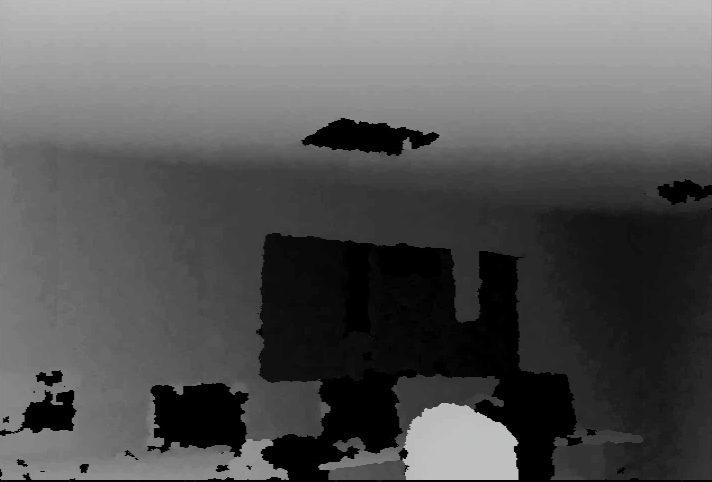
\includegraphics[width=0.25\textwidth]{figuras/5.Testes/deteccao/1.png}}
				\subfloat[] {
					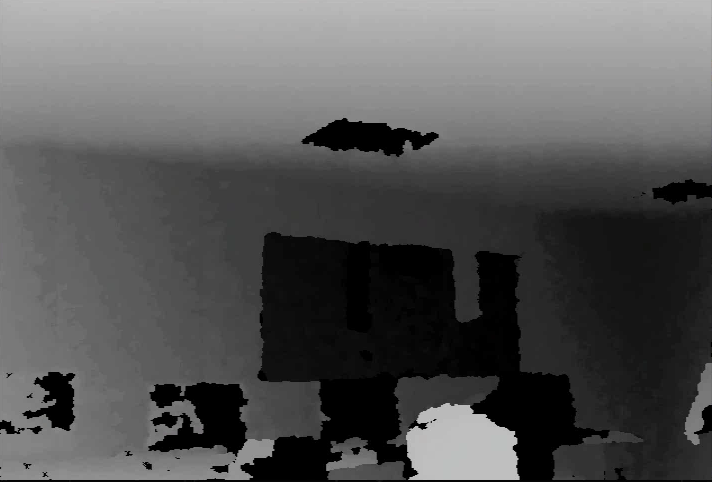
\includegraphics[width=0.25\textwidth]{figuras/5.Testes/deteccao/2.png}}
				\subfloat[] {
					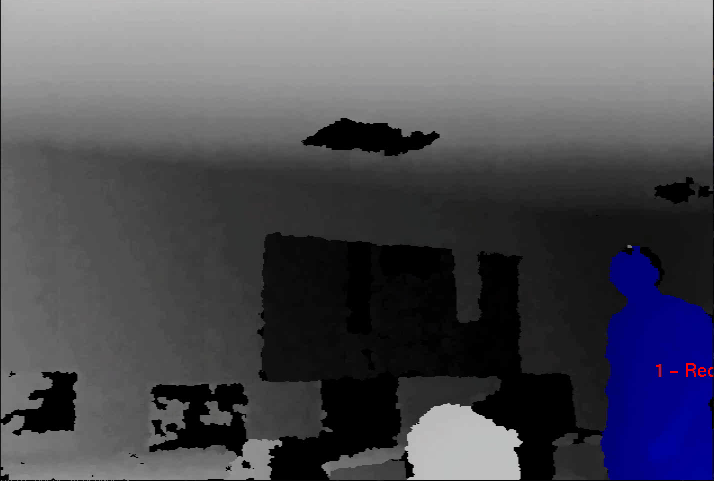
\includegraphics[width=0.25\textwidth]{figuras/5.Testes/deteccao/3.png}}
				\subfloat[] {
					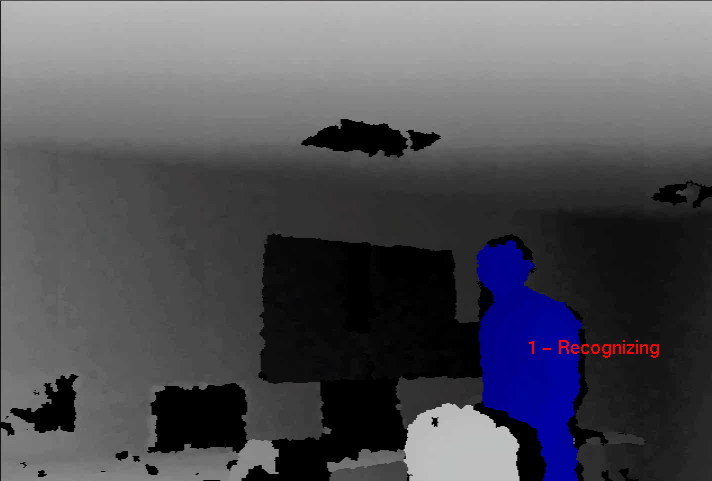
\includegraphics[width=0.25\textwidth]{figuras/5.Testes/deteccao/4.png}}
			\end{center}
			\caption{Detecção de novos usuários.}
			\label{fig:testes_deteccao}
		\end{figure}
		
	\subsection{Testes do Máximo de Usuários}
	
		% TODO : Escrever e adicionar imagens sobre o máximo de usuários possíveis na
		% cena.
	
	\subsection{Teste de Oclusão}
	
		Um problema conhecido e previsto é a oclusão. O problema foi tratado da melhor
		forma possível mas como o Sistema TRUE foi elaborado com apenas um Kinect a
		sua abrangência ficou comprometida. Na Figura \ref{fig:testes_oclusao}
		é exemplificado o tratamento da oclusão, onde, por alguns instantes, o usuário
		se perde na cena. A Figura \ref{fig:testes_oclusao_ocluso} mostra o usuário
		saindo da sua situação de oclusão e ainda não foi detectado pelo TRUE. Outro
		exemplo é o da Figura \ref{fig:testes_oclusao_sucesso}.
	
		\begin{figure}[H]
		\begin{center}
				\subfloat[] {
					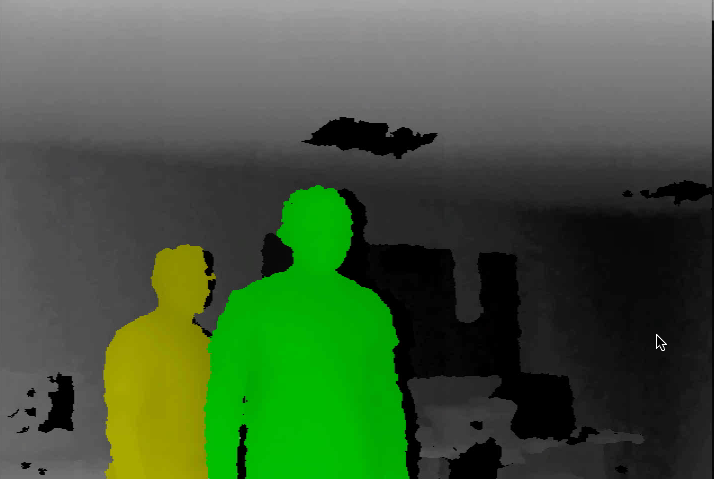
\includegraphics[width=0.19\textwidth]{figuras/5.Testes/oclusao/1.png}}
				\subfloat[] {
					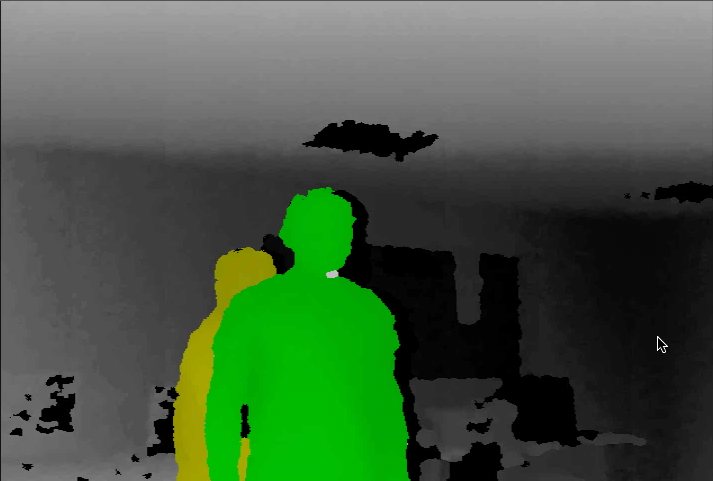
\includegraphics[width=0.19\textwidth]{figuras/5.Testes/oclusao/2.png}}
				\subfloat[] {
					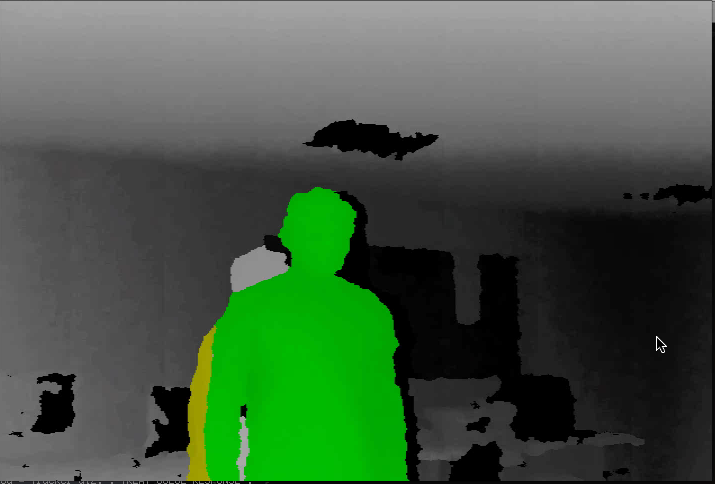
\includegraphics[width=0.19\textwidth]{figuras/5.Testes/oclusao/3.png}}
				\subfloat[] {
					\label{fig:testes_oclusao_ocluso}
					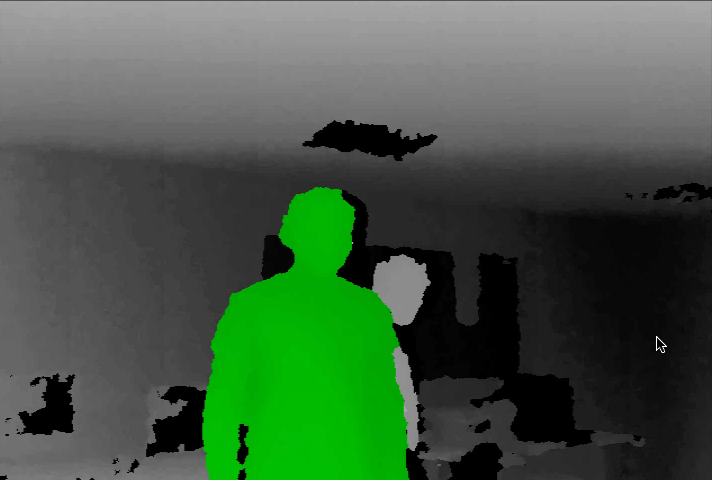
\includegraphics[width=0.19\textwidth]{figuras/5.Testes/oclusao/4.png}}
				\subfloat[] {
					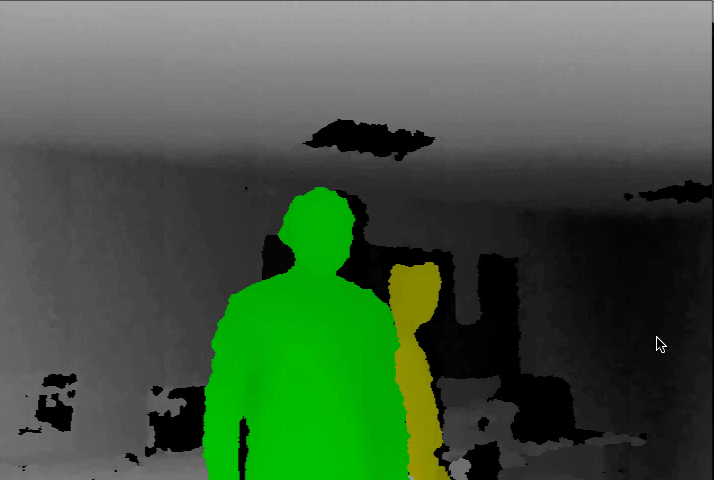
\includegraphics[width=0.19\textwidth]{figuras/5.Testes/oclusao/5.png}}
			\end{center}
			\caption{Oclusão de usuários.}
			\label{fig:testes_oclusao}
		\end{figure}
		
		
		\begin{figure}[H]
			\begin{center}
				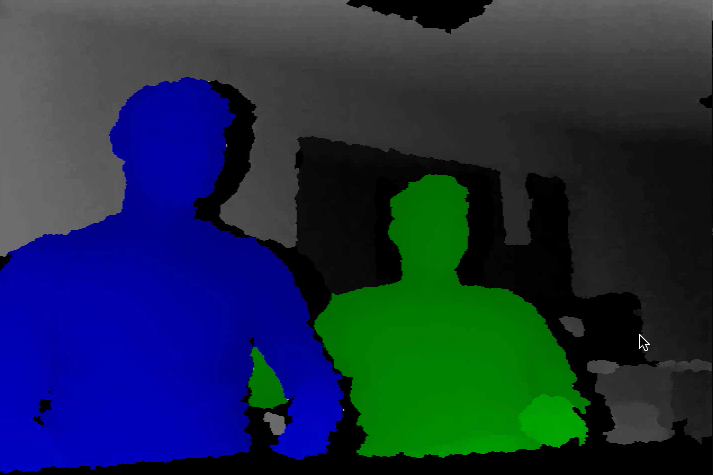
\includegraphics[width=0.75\textwidth]{figuras/5.Testes/oclusao/oclusao_corretamente.png}
			\end{center}
			\caption{Oclusão de usuários ocorrendo com sucesso.}
			\label{fig:testes_oclusao_sucesso}
		\end{figure}
		
	
	\subsection{Testes de Relacionamento com Objetos}
	
		Outro erro conhecido é o que acontece quando o usuários se relaciona com
		objetos no ambiente. Quando isso acontece o Sistema TRUE não sabe separa a
		area do usuário da area do objeto e por isso gera os
		erros exemplificados na Figura \ref{fig:testes_relacionamento_com_objetos}.
	
		\begin{figure}[H]
			\begin{center}
				\subfloat[] {
					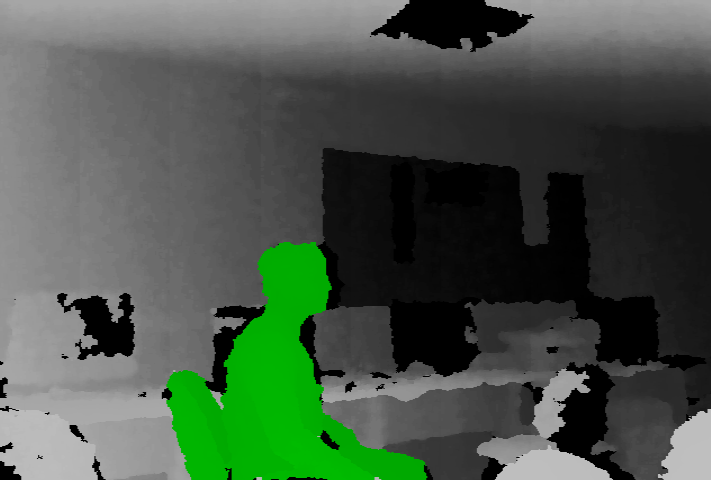
\includegraphics[width=0.37\textwidth]{figuras/5.Testes/relacionamento_com_objetos/1.png}}
				\subfloat[] {
					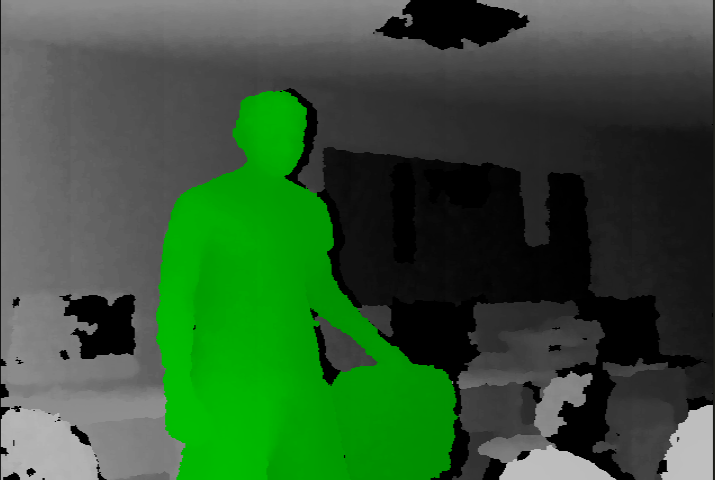
\includegraphics[width=0.37\textwidth]{figuras/5.Testes/relacionamento_com_objetos/2.png}}
			\end{center}
			\caption{Usuários sendo rastreado conjuntamente com os objetos que
			interagem.}
			\label{fig:testes_relacionamento_com_objetos}
		\end{figure}
		
	
	\subsection{Testes de Interferência}
	
		Similar ao erro acima, a interferência gerada entre um usuário no outro é
		exemplificado na Figura \ref{fig:testes_relacionamento_com_usuarios} onde
		partes de um usuário são confundidas com outro usuário.

		\begin{figure}[H]
			\begin{center}
				\subfloat[] {
					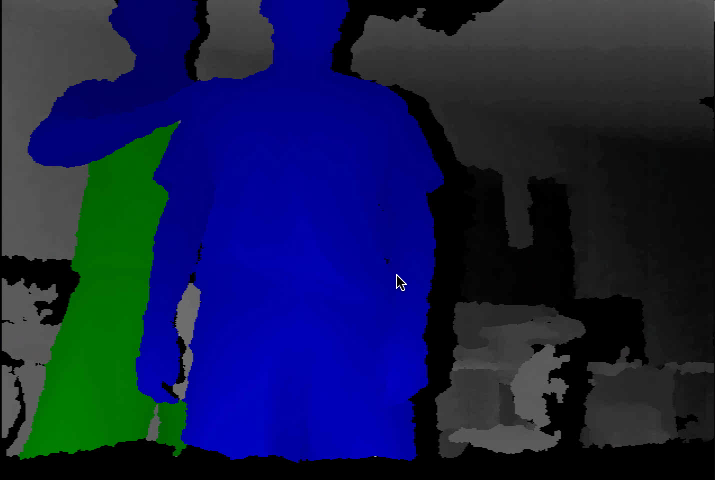
\includegraphics[width=0.32\textwidth]{figuras/5.Testes/relacionamento_com_pessoas/1.png}}
				\subfloat[] {
					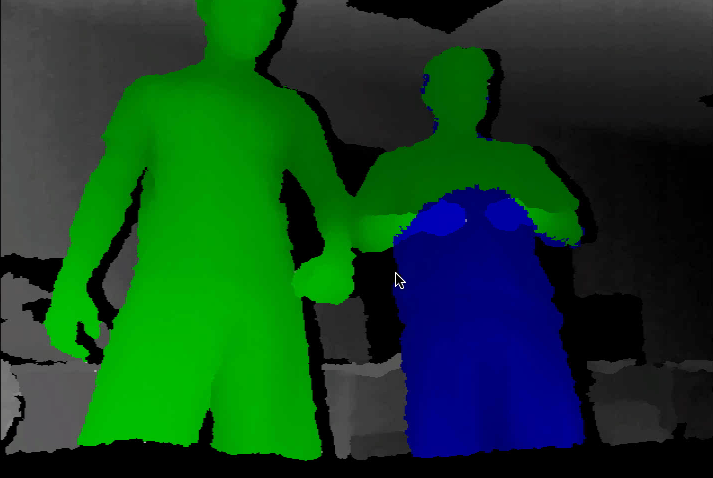
\includegraphics[width=0.32\textwidth]{figuras/5.Testes/relacionamento_com_pessoas/2.png}}
				\subfloat[] {
					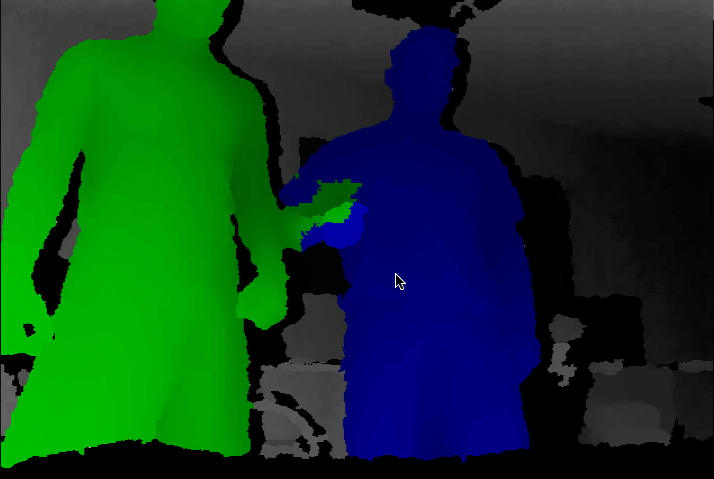
\includegraphics[width=0.32\textwidth]{figuras/5.Testes/relacionamento_com_pessoas/3.png}}
			\end{center}
			\caption{Usuários sofrendo interferência dos que estão ao seu redor.}
			\label{fig:testes_relacionamento_com_usuarios}
		\end{figure}
		
		
Apesar do pesares apresentados anteriormente o rastreamento apresentou uma
excelente performance e correspondeu ao esperado. 
	